%!TEX root = ../../thesis.tex

For a particle to be considered ``discovered'' within the particle physics community, 
convention requires the null hypothesis to be rejected with $5\sigma$ significance, 
corresponding to $<0.0001\%$ chance that the observation is a statistical fluctuation.
In the summer of 2012, this level of significance was reached independently by the ATLAS 
and CMS collaborations, primarily driven by searches for \HepProcess{\PHiggs \HepTo 
\Pphoton\Pphoton} and \HepProcess{\PHiggs \HepTo \PZ\PZ} and supported by the \HWW search 
\cite{ATLAS-discovery,CMS-discovery}. Both experiments observed a resonance at 
\unit{$m \approx 125$}{\GeV}.

This observation was quickly corroborated by a combination of \HepProcess{\PV\PHiggs 
\HepTo \PV\Pbottom\APbottom} searches performed by the CDF and \dzero experiments at the 
Tevatron, which yielded consistent results with $3.1\sigma$ significance 
\cite{Tevatron:2012}.

Using the entire Run I dataset, the significance of the particle discovery was extended 
by the ATLAS experiment to $7.4\sigma$ in \HepProcess{\PHiggs \HepTo \Pphoton\Pphoton} 
\cite{ATLAS:combination:2013}, $6.6\sigma$ in \HepProcess{\PHiggs \HepTo \PZ\PZ} 
\cite{ATLAS:combination:2013}, and $5\sigma$\todo{update} in \HWW (see 
\Chapter~\ref{chap:results}). Focus inevitably shifted to measuring its properties (mass, 
couplings, spin, parity) in order to test the hypothesis that it is the SM Higgs boson.
Thus far, all experimental measurements have supported this hypothesis.



\subsection{Mass measurement}
\label{sec:searches:mass}

The mass of the Higgs boson, \mH, is unpredicted by the SM, and is very important to 
measure precisely. Once \mH is known, all the Higgs boson couplings, production cross 
sections and branching ratios can be calculated (see \Section~\ref{sec:properties}). The 
value of \mH is also important when assessing the theoretical implications of the 
discovery (see \Section~\ref{sec:implications}).

The \HepProcess{\PHiggs \HepTo \Pphoton\Pphoton} and \HepProcess{\PHiggs \HepTo \PZ\PZ} 
decay channels offer the best sensitivity to \mH, since they exhibit very clean 
experimental signatures and can fully reconstruct the Higgs boson four-momentum.
Combining these two channels gives an \mH measurement of 
\unit{\statsyst{125.5}{0.2}{0.6}{}}{\GeV} in ATLAS \cite{ATLAS:combination:2013} and 
\unit{\statsyst{125.7}{0.3}{0.3}{}}{\GeV} in CMS \cite{CMS:mass}. These are in excellent 
agreement, although some tension exists between the two ATLAS channels.

Nature has been kind in providing a Higgs boson with \unit{$\mH \approx 126$}{\GeV}, 
since many different production modes and decay channels should be experimentally 
accessible at the LHC (see Figures~\ref{fig:higgs_xs} and \ref{fig:higgs_br}). In 
particular, couplings to bosons and fermions can be measured, providing evidence of the 
two types of mass generation that the Higgs field is responsible for in the SM.



\subsection{Coupling measurements and limits}
\label{sec:searches:couplings}

Coupling strengths of the Higgs boson to other SM particles are probed by searching for 
different experimental signatures, which correspond to specific combinations of 
production mode and decay channel. For example, the \WH production mode with the \HWW 
decay mode is sensitive only to the \HepProcess{\PHiggs\PW\PW} coupling. On the other 
hand, the ggF production mode and the \HepProcess{\PHiggs \HepTo \Pphoton\Pphoton} decay 
channel feature loops, and interpreting results in terms of couplings is less 
straightforward. Undiscovered massive particles may contribute to such loops, distorting 
the effective coupling to gluons and photons.

Measurements of \HepProcess{\PHiggs \HepTo \Pphoton\Pphoton}, \HepProcess{\PHiggs \HepTo 
\PZ\PZ}, \HWW and \HepProcess{\PHiggs \HepTo \Ptau\Ptau} were made with the Run I 
dataset, with signal regions optimised for ggF and VBF production. A measurement of 
\HepProcess{\PV\PHiggs \HepTo \PV\Pbottom\APbottom} was also made. Assuming SM couplings, 
the measured cross sections can be expressed as a signal strength $\mu = 
\sigma_{\text{meas}} / \sigma_{\text{SM}}$. The signal strengths measured with the ATLAS 
experiment are consistent with the SM, as shown in \Figure~\ref{fig:concl:mu}.
Similar measurements were made with the CMS detector, also yielding signal strengths 
compatible with the SM \cite{CMS:Hgamgam,CMS:HZZ,CMS:HWW,CMS:Htautau,CMS:Hbb}.

\begin{figure}[t]
	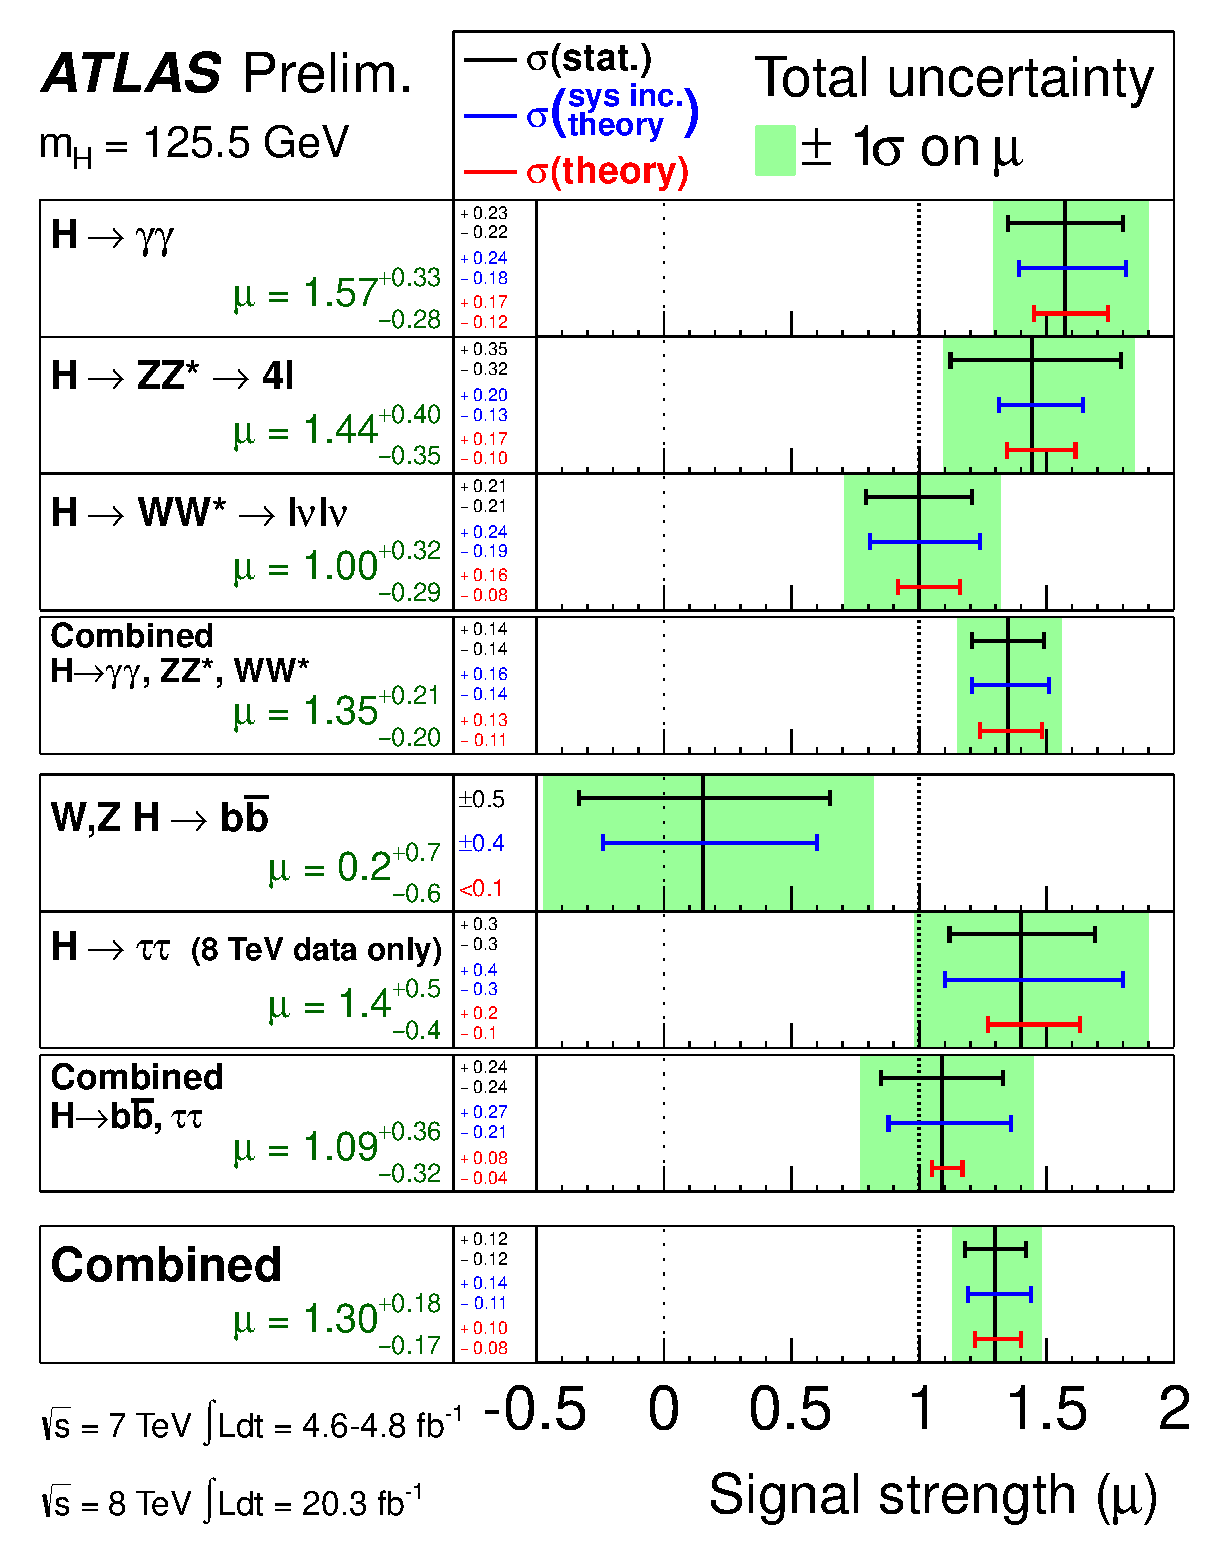
\includegraphics[width=\mediumfigwidth]{tex/conclusions/atlas_mu}
	\caption{Measured signal strength (\unit{$\mH = 125.5$}{\GeV}) for each final state 
	\cite{ATLAS:couplings:Moriond14}. Combinations of bosonic, fermionic and all decay 
	channels are also shown. The \HWW result is from a previous analysis version.}
	\label{fig:concl:mu}
\end{figure}

It is also informative to split the signal strength according to the production mode. 
\Figure~\ref{fig:concl:mu_2D} shows the likelihood contours for a fit with two signal 
strength parameters: one for production modes dominated by a fermionic coupling (ggF and 
\ttH), and the other for those dominated by a bosonic coupling (VBF and \VH). Again, this 
does assume the couplings themselves are those predicted by the SM. However, it is useful 
to see which analyses are sensitive to which types of couplings. It is clear that \HWW is 
a very sensitive analysis for couplings measurements.

\begin{figure}[t]
	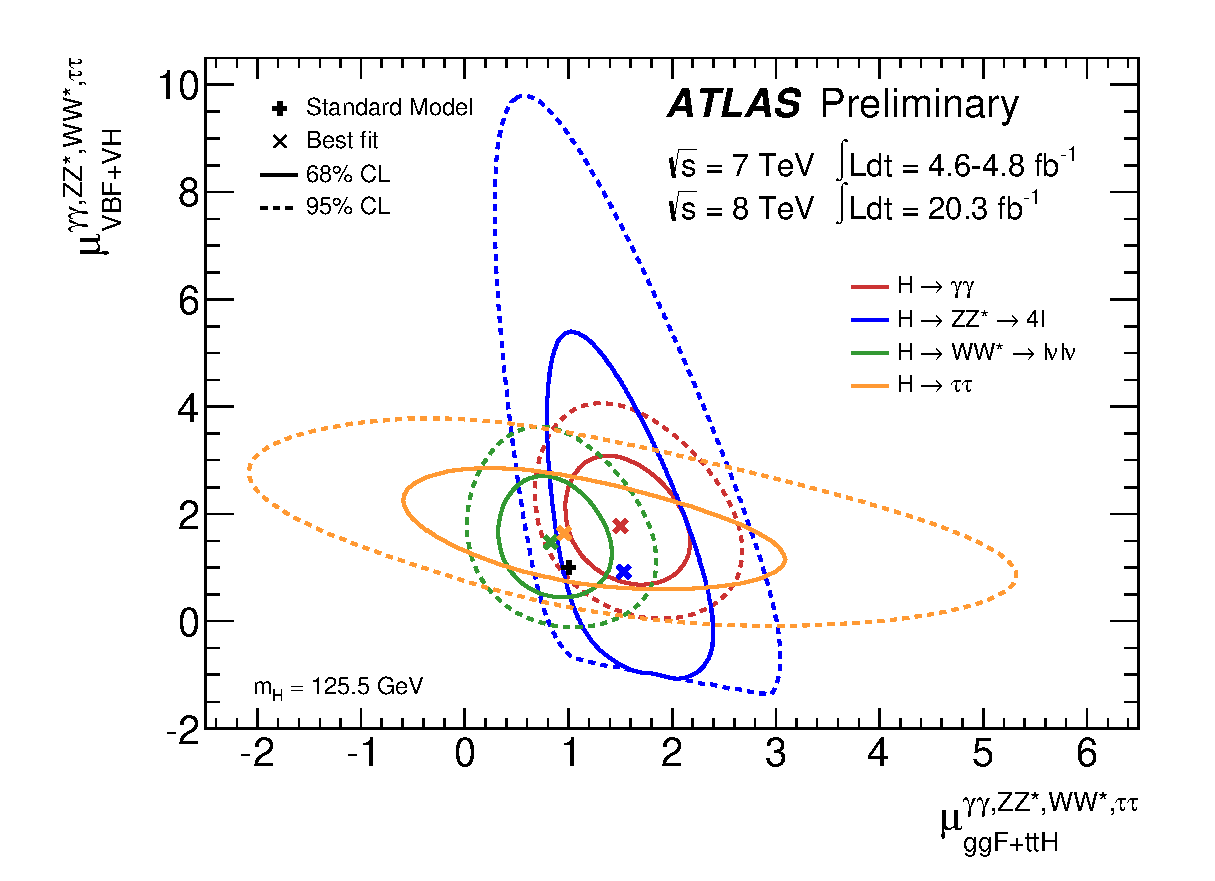
\includegraphics[width=\largefigwidth]{tex/conclusions/atlas_mu_2D}
	\caption{Likelihood contours of measured signal strength (\unit{$\mH = 125.5$}{\GeV}) 
	for each final state \cite{ATLAS:couplings:Moriond14}. Signal strengths are split 
	according to the dominant coupling in the production mode: fermionic (ggF and \ttH) 
	or bosonic (VBF and \VH). The \HWW result is from a previous analysis version.}
	\label{fig:concl:mu_2D}
\end{figure}

These measurements were used to test specific coupling scenarios in 
\Reference~\cite{ATLAS:couplings:Moriond14}, though no significant deviations from the SM 
were observed. The two most generic scenarios are highlighted here. 

The first scenario assumes a SM particle content. The probed couplings are free 
parameters in the fit, and are expressed as coupling scale factors: 
$\kappa_{\PZ}, \kappa_{\PW}, \kappa_{\Ptop}, \kappa_{\Pbottom}, \kappa_{\Ptau}$. The 
\HepProcess{\PHiggs\Pphoton\Pphoton} and \HepProcess{\PHiggs\Pgluon\Pgluon} effective 
couplings and the total width are then calculated within the framework of the SM, as 
functions of the $\kappa_i$. Compatibility with the SM is $p = 0.13$ (see 
\Figure~\ref{fig:concl:couplings:SM}), with differences driven by the measured 
\HepProcess{\PHiggs \HepTo \Pbottom\APbottom} cross section.

The second scenario allows for undiscovered particles, which may contribute through loops 
or to the total width. Thus, two effective coupling scale factors are introduced 
($\kappa_{\Pphoton}, \kappa_{\Pgluon}$), while the absence of a total width constraint 
means that only coupling ratios can be probed. The free parameters of the fit are 
$\lambda_{\Pphoton\PZ}, \lambda_{\PW\PZ}, \lambda_{\Pbottom\PZ}, \lambda_{\Ptau\PZ}, 
\lambda_{\Pgluon\PZ}, \lambda_{\Ptop\Pgluon}, \kappa_{\Pgluon\PZ}$ where 
$\lambda_{ij} = \kappa_i / \kappa_j$, $\kappa_{ij} = \kappa_i \cdot \kappa_j / 
\kappa_{\PHiggs}$ and $\kappa_{\PHiggs}$ is the scale factor of the total width. 
Compatibility with the SM is $p = 0.21$ (see \Figure~\ref{fig:concl:couplings:BSM}). The 
large uncertainty on $\lambda_{\Ptop\Pgluon}$ could be improved by a measurement of the 
\ttH production mode.

\begin{figure}[t]
	\begin{subfigure}[b]{0.495\textwidth}
		\centering
		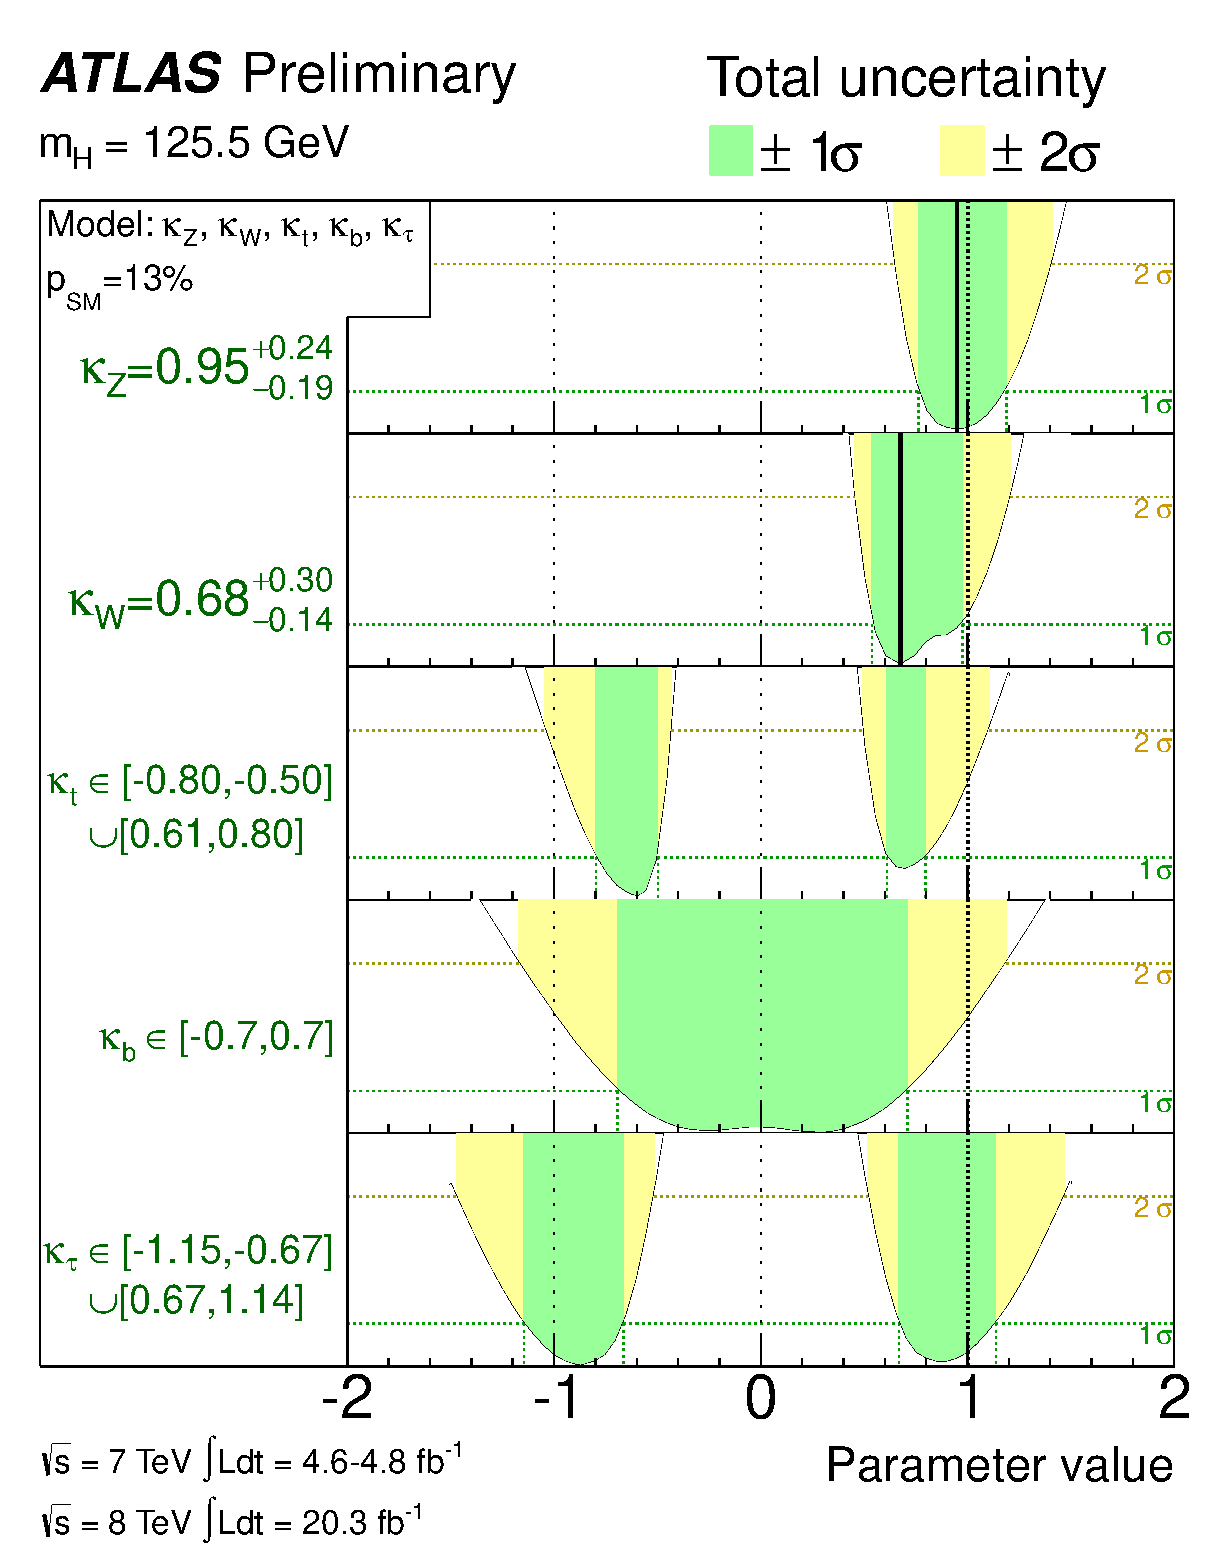
\includegraphics[width=\textwidth]{tex/conclusions/atlas_couplings_SM}
		\caption{SM particle content}
		\label{fig:concl:couplings:SM}
	\end{subfigure}
	\hfill
	\begin{subfigure}[b]{0.495\textwidth}
		\centering
		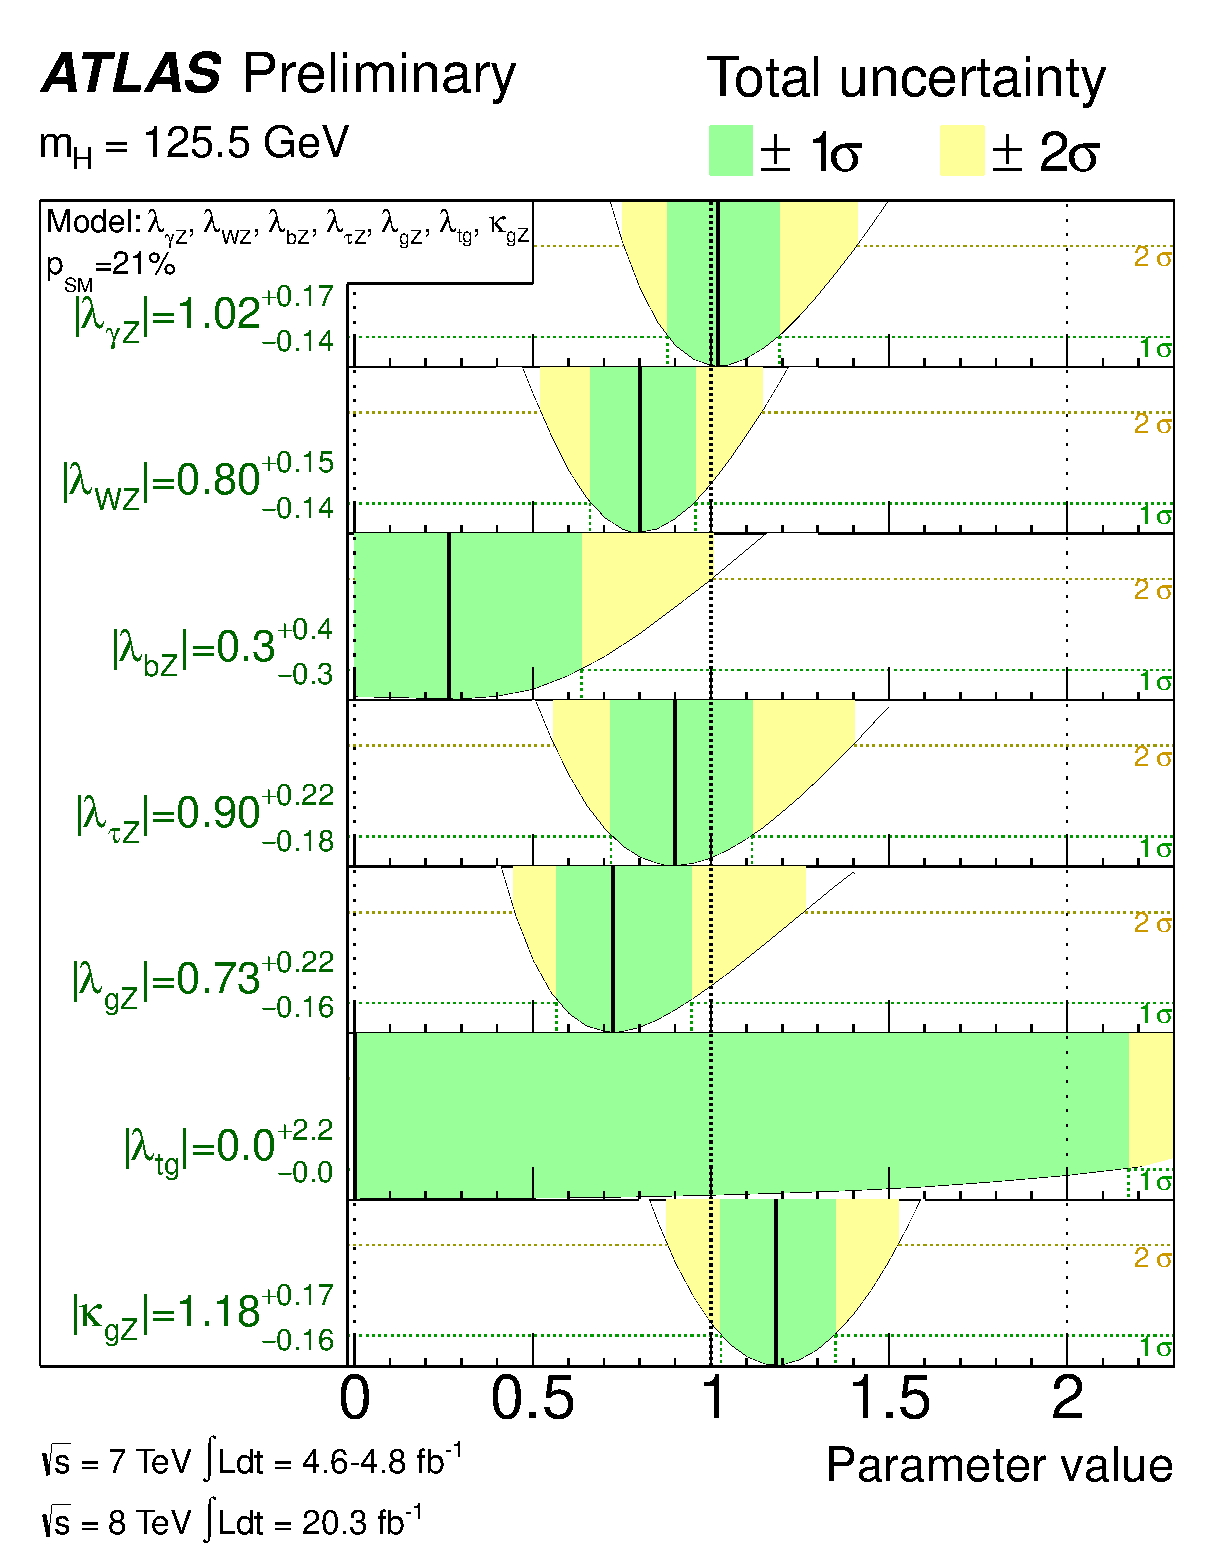
\includegraphics[width=\textwidth]{tex/conclusions/atlas_couplings_BSM}
		\caption{SM + undiscovered particle content}
		\label{fig:concl:couplings:BSM}
	\end{subfigure}
	\caption{Measured likelihood curves of coupling scale factors $\kappa_i$ and ratios 
	$\lambda_{ij} = \kappa_i / \kappa_j$, for two generic models described in the text 
	\cite{ATLAS:couplings:Moriond14}.}
	\label{fig:concl:couplings}
\end{figure}

In addition to the five measured channels described above, upper bounds on other decay 
channels have also been set. The observed limits at \unit{$\mH = 125$}{\GeV} are 
$\sigma < 11\sigma_{\text{SM}}$ for \HepProcess{\PHiggs \HepTo \PZ\Pphoton} 
\cite{ATLAS:HZgam} and $\sigma < 10\sigma_{\text{SM}}$ for \HepProcess{\PHiggs \HepTo 
\Pmu\Pmu} \cite{ATLAS:Hmumu}, at the 95\% CL. Also, a search for \HepProcess{\ZH \HepTo 
\Plepton\Plepton\met} has constrained the branching ratio to invisible particles to 
$< 75\%$ at the 95\% CL, assuming $\sigma = \sigma_{\text{SM}}$ and 
\unit{$\mH = 125$}{\GeV} \cite{ATLAS:Hinv}. Such a limit is important because 
undiscovered massive particles (dark matter candidates) could enhance the invisible width 
$\Gamma_{\text{inv}}$. Similar limits have been set by the CMS collaboration 
\cite{CMS:HZgam,CMS:Hmumu,CMS:Hinv}.



\subsection{Spin and parity measurement}
\label{sec:searches:spin}

The SM Higgs boson is a spin-0 and CP-even particle, \ie $J^P = 0^+$. It is important to 
experimentally confirm these properties, in order to establish that the observed particle 
is the Higgs boson. According to the Landau-Yang theorem, the spin-1 hypothesis is 
excluded by the observation of \HepProcess{\PHiggs \HepTo \Pphoton\Pphoton} 
\cite{Landau:1948,Yang:1950}. Nevertheless, it can still be tested by the other channels.

The $J^P$ was probed by considering the decay topologies of events in the 
\HepProcess{\PHiggs \HepTo \PZ\PZ}, \HWW and \HepProcess{\PHiggs \HepTo \Pphoton\Pphoton} 
measurements with ATLAS. However, some event selection criteria were altered with respect 
to the coupling measurements, in order to reduce bias. For example, the \HWW selection 
exploits the spin-0 hypothesis in the \unit{$\mll < 55$}{\GeV} and $\dphill < 1.8$ 
criteria (see \Chapter~\ref{chap:selection}).

The $0^-, 1^+, 1^-, 2^+$ hypotheses are excluded at greater than 97.8\% CL, whilst the 
data are compatible with the $0^+$ hypothesis \cite{ATLAS:spin}. This provides strong 
evidence that the discovered particle is spin-0. The discovered particle could be a 
mixture of CP-even and CP-odd states, though a preference for CP-even is observed.


